\pdfminorversion=4
\documentclass[aspectratio=169]{beamer}

\mode<presentation>
{
  \usetheme{default}
  \usecolortheme{default}
  \usefonttheme{default}
  \setbeamertemplate{navigation symbols}{}
  \setbeamertemplate{caption}[numbered]
  \setbeamertemplate{footline}[frame number]  % or "page number"
  \setbeamercolor{frametitle}{fg=white}
  \setbeamercolor{footline}{fg=black}
} 

\usepackage[english]{babel}
\usepackage[utf8x]{inputenc}
\usepackage{tikz}
\usepackage{courier}
\usepackage{array}
\usepackage{bold-extra}
\usepackage{minted}
\usepackage[thicklines]{cancel}
\usepackage{fancyvrb}
\usepackage{tabto}

\xdefinecolor{dianablue}{rgb}{0.18,0.24,0.31}
\xdefinecolor{darkblue}{rgb}{0.1,0.1,0.7}
\xdefinecolor{darkgreen}{rgb}{0,0.5,0}
\xdefinecolor{darkgrey}{rgb}{0.35,0.35,0.35}
\xdefinecolor{darkorange}{rgb}{0.8,0.5,0}
\xdefinecolor{darkred}{rgb}{0.7,0,0}
\definecolor{darkgreen}{rgb}{0,0.6,0}
\definecolor{mauve}{rgb}{0.58,0,0.82}

\title[2019-06-19-nyu-as-jimstuff]{``Jim stuff''}
\author{Jim Pivarski}
\institute{Princeton University -- IRIS-HEP}
\date{June 19, 2019}

\usetikzlibrary{shapes.callouts}

\begin{document}

\logo{\pgfputat{\pgfxy(0.11, 7.4)}{\pgfbox[right,base]{\tikz{\filldraw[fill=dianablue, draw=none] (0 cm, 0 cm) rectangle (50 cm, 1 cm);}\mbox{\hspace{-8 cm}
\includegraphics[height=1 cm]{princeton-logo-long.png}\hspace{0.1 cm}\raisebox{0.1 cm}{
\includegraphics[height=0.8 cm]{iris-hep-logo-long.png}}\hspace{0.1 cm}}}}}

\begin{frame}
  \titlepage
\end{frame}

\logo{\pgfputat{\pgfxy(0.11, 7.4)}{\pgfbox[right,base]{\tikz{\filldraw[fill=dianablue, draw=none] (0 cm, 0 cm) rectangle (50 cm, 1 cm);}\mbox{\hspace{-8 cm}
\includegraphics[height=1 cm]{princeton-logo.png}\hspace{0.1 cm}\raisebox{0.1 cm}{
\includegraphics[height=0.8 cm]{iris-hep-logo.png}}\hspace{0.1 cm}}}}}

% Uncomment these lines for an automatically generated outline.
%\begin{frame}{Outline}
%  \tableofcontents
%\end{frame}

% START START START START START START START START START START START START START

\begin{frame}{Apologies for any misrepresentation}
\vspace{0.1 cm}
\begin{columns}
\column{1.15\linewidth}
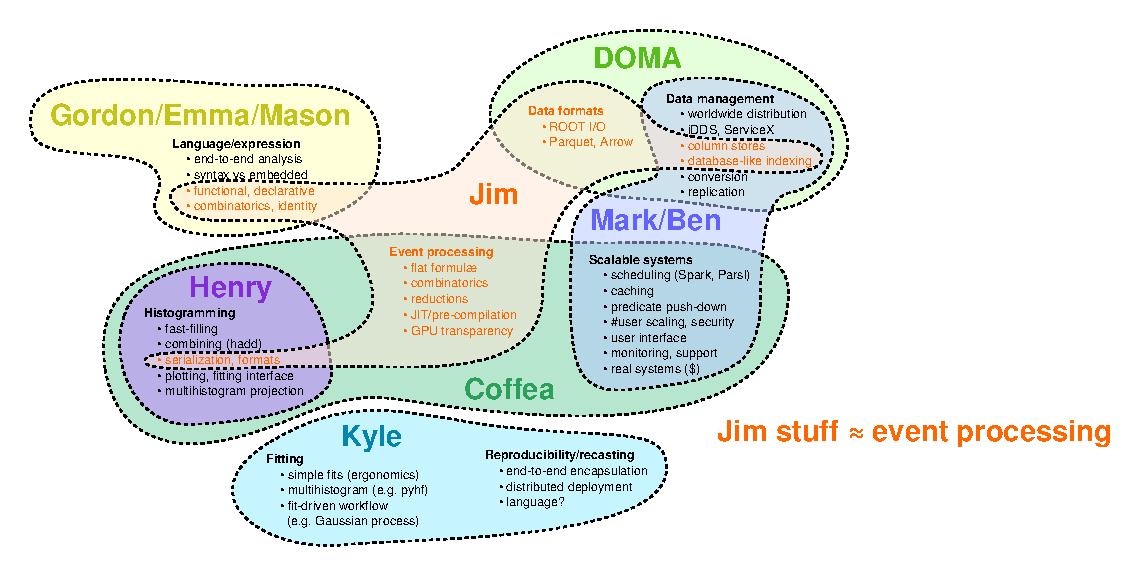
\includegraphics[width=\linewidth]{everybody.pdf}
\end{columns}
\end{frame}

\begin{frame}{Projects and collaborations}
\vspace{0.5 cm}
\begin{columns}
\column{1.15\linewidth}
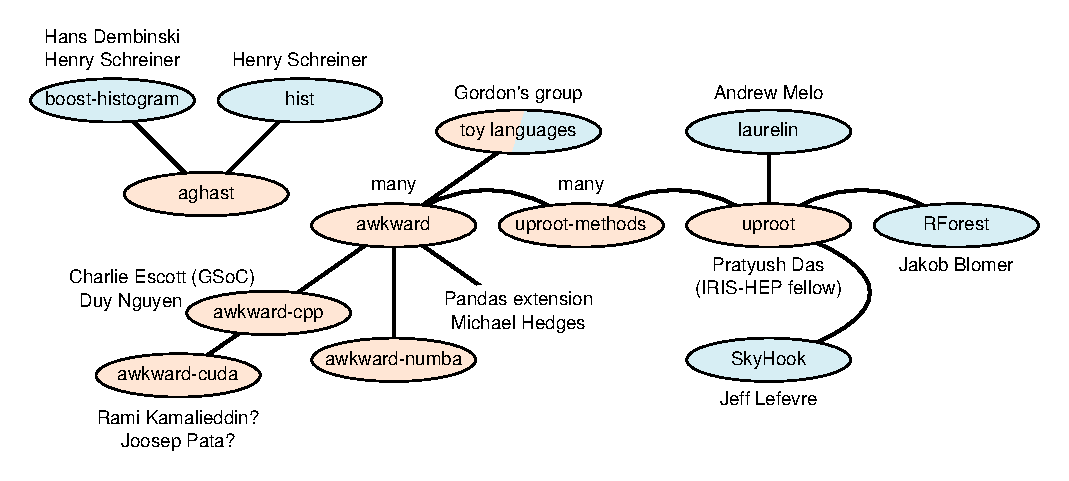
\includegraphics[width=\linewidth]{projects.pdf}
\end{columns}
\end{frame}

\begin{frame}{Year of teaching}
\vspace{0.5 cm}
\large

\begin{itemize}\setlength{\itemsep}{0.25 cm}
\item \textcolor{darkblue}{April 1:}     \tabto{2.3 cm}Software Carpentry at Fermilab (intensity frontier)
\item \textcolor{darkblue}{April 8--10:} \tabto{2.3 cm}PICSciE Numpy course at Princeton (mostly science)
\item \textcolor{darkblue}{May 6:}       \tabto{2.3 cm}Language tools tutorial at ADL workshop (particle physics)
\item \textcolor{darkblue}{May 28--29:}  \tabto{2.3 cm}Scientific Python and columnar analysis HATS (CMS)
\item \textcolor{darkblue}{June 10:}     \tabto{2.3 cm}Software Carpentry at Argonne (U.S.\ ATLAS)
\item \textcolor{darkblue}{July 22--26:} \tabto{2.3 cm}CoDaS-HEP (particle physics)
\end{itemize}

\vspace{0.5 cm}
\begin{itemize}
\item Pratyush Das (IRIS-HEP fellow)
\item Charlie Escott (GSoC)
\item Duy Nguyen (volunteer)
\end{itemize}
\end{frame}

\begin{frame}{Keeping up with uproot}
\vspace{0.5 cm}

\only<1>{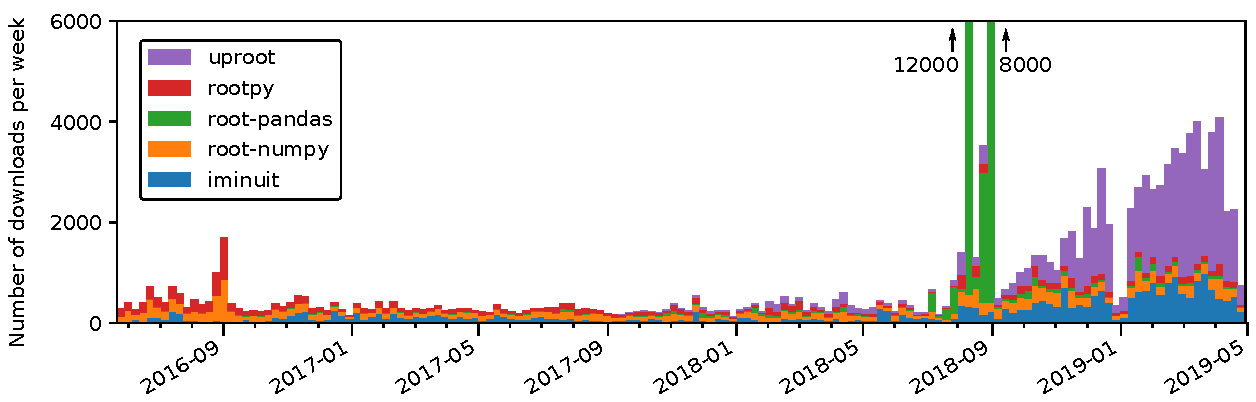
\includegraphics[width=\linewidth]{all_file_project.pdf}}\only<2>{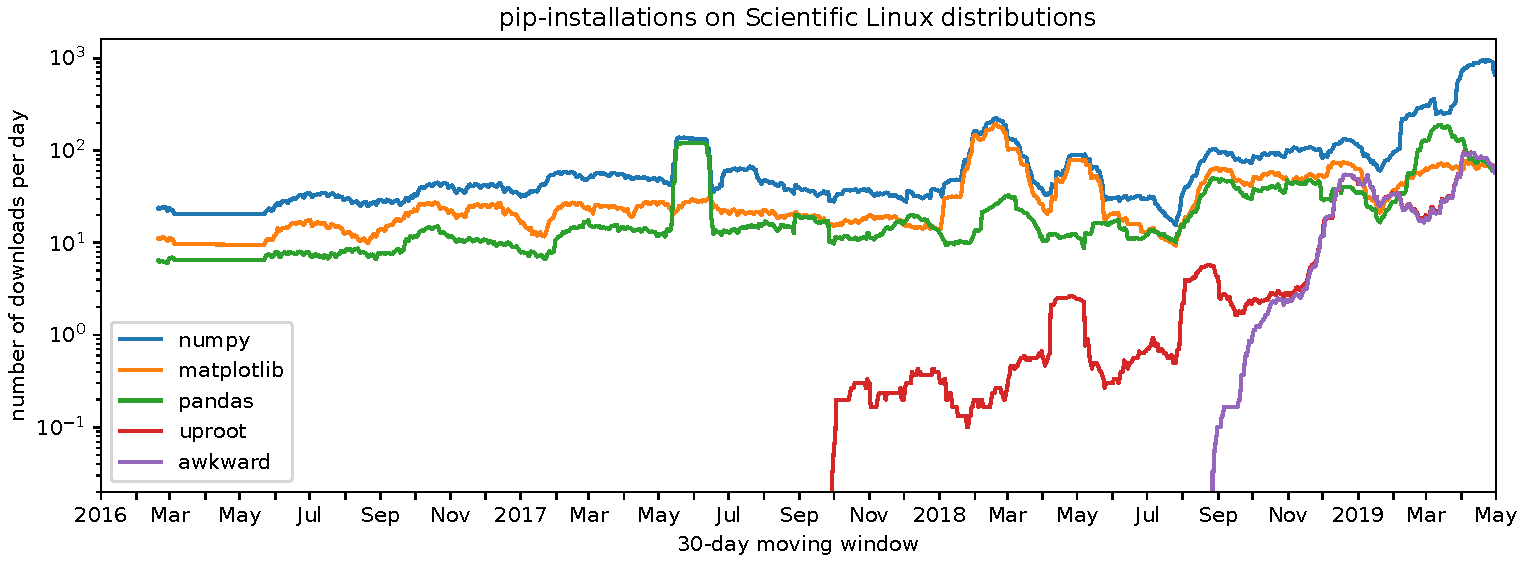
\includegraphics[width=\linewidth]{pip-scientificlinux-uproot.pdf}}

\only<1>{\vspace{0.65 cm}}
\begin{itemize}
\item Uproot is wildly popular {\tt:)}
\item Nobody (except Coffea) installs awkward-array on its own, only through uproot {\tt:(}
\item The way to get new awkward features in front of a lot of physicists is to make it an option in uproot.
\end{itemize}
\end{frame}

\begin{frame}[fragile]{Lazy arrays in uproot (ChunkedArrays of VirtualArrays in awkward)}
\large
\vspace{0.25 cm}

Lazy arrays have an interface like direct arrays but internally iterate in chunks.

\small
\begin{minted}{python}
>>> ttree.array("Muon_pt")      # loads whole array, contiguously
\end{minted}

\vspace{-0.6 cm}
\color{darkblue}\begin{verbatim}
<JaggedArray  [[] [] [5.31576] ... [26.35128] [] [44.2805 6.699721]]>
\end{verbatim}
\color{black}

\vspace{-0.6 cm}
\begin{minted}{python}
>>> ttree.lazyarray("Muon_pt")  # loads first and last chunk (to print)
\end{minted}

\vspace{-0.6 cm}
\color{darkblue}\begin{verbatim}
<ChunkedArray [[] [] [5.31576] ... [26.35128] [] [44.2805 6.699721]]>
\end{verbatim}
\color{black}\large

\begin{uncoverenv}<2->
The following splits data into 1~GB chunks, loading no more than 3~GB at a time, and computes \mintinline{python}{pz} from \mintinline{python}{Muon_pt} and \mintinline{python}{Muon_eta}.

\small
\begin{minted}{python}
>>> cache = uproot.ArrayCache("3 GB")
>>> events = uproot.lazyarrays("cms-nanoaod/*.root", "Events",
                               entrysteps="1 GB", cache=cache)
>>> pz = events.Muon_pt * numpy.sinh(events.Muon_eta)
\end{minted}
\end{uncoverenv}
\end{frame}

\begin{frame}[fragile]{Lazy profile: CMS NanoAOD}
\large
\vspace{0.5 cm}

\begin{columns}
\column{1.05\linewidth}
If your TTrees are CMS NanoAOD, you can get lazy arrays as an event hierarchy:

\small
\begin{minted}{python}
>>> events = ttree.lazyarrays(profile="cms.nanoaod")
>>> events
\end{minted}

\vspace{-0.6 cm}
\color{darkblue}\begin{verbatim}
<Table [<Event 0> <Event 1> ... <Event 499998> <Event 499999>]>
\end{verbatim}
\color{black}

\vspace{-0.6 cm}
\begin{minted}{python}
>>> events.muons           # now it reads nMuon...
\end{minted}

\vspace{-0.6 cm}
\color{darkblue}\begin{verbatim}
<ChunkedArray [[] [] [<Muon 0>] ... [] [<Muon 537187> <Muon 537188>]]>
\end{verbatim}
\color{black}

\vspace{-0.6 cm}
\begin{minted}{python}
>>> events.muons.pt        # now it reads Muon_pt...
\end{minted}

\vspace{-0.6 cm}
\color{darkblue}\begin{verbatim}
<ChunkedArray [[] [] [5.315762] ... [] [44.28051 6.6997213]]>
\end{verbatim}
\color{black}

\vspace{-0.6 cm}
\begin{minted}{python}
>>> events.columns         # to see structure (also tab-complete)
\end{minted}

\vspace{-0.6 cm}
\color{darkblue}\begin{verbatim}
['run', 'lumi', 'event', 'electrons', 'muons', 'taus', 'photons',
 'jets', 'fatjets', 'subjets', 'isotracks', 'softjets', 'softactivity',
 'fixedGridRhoFastjet', 'MET', 'rawMET', 'caloMET', 'puppiMET', 'tkMET',
 'PV', 'SVs', 'otherPVs', 'pileup', 'trigobjs', 'gen', 'etc', 'raw']
\end{verbatim}
\color{black}

\vspace{-0.6 cm}
\begin{minted}{python}
>>> events.muons.columns   # to see the muon columns...
\end{minted}
\end{columns}
\end{frame}

\begin{frame}[fragile]{Lazy profile: CMS NanoAOD}
\large
\vspace{0.3 cm}

Since everything is loaded on demand, some fields can be defined in terms of others without unnecessary reading or memory use.

\small
\begin{minted}{python}
>>> events.muons.p4     # now it reads Muon_eta, Muon_phi, Muon_mass
\end{minted}

\vspace{-0.4 cm}
\color{darkblue}\begin{verbatim}
<ChunkedArray [[] []
               [TLorentzVector(5.315, 1.127, 2.695, 0.1057)]
               ...
               [TLorentzVector(44.281, 0.7856,  2.3838, 0.10571)
                TLorentzVector(6.6997, 1.9197, -0.0706, 0.10571)]]>
\end{verbatim}
\color{black}\large

\begin{uncoverenv}<2->
Cross-references are presented as objects, too.

\small
\begin{minted}{python}
>>> events.muons.jet    # now it reads Muon_JetIdx and nJet
\end{minted}

\vspace{-0.3 cm}
\color{darkblue}\begin{verbatim}
<ChunkedArray [[] [] [<Jet 12>] ... [<Jet 4102602> <Jet 4102603>]]>
\end{verbatim}
\color{black}\large
\end{uncoverenv}

\begin{uncoverenv}<3->
So we can compute things like ``$\Delta \phi$ between every muon and its associated jet.''

\small
\begin{minted}{python}
>>> events.muons.p4.delta_phi(events.muons.jet.p4)
\end{minted}

\vspace{-0.3 cm}
\color{darkblue}\begin{verbatim}
<ChunkedArray [[] [] [-0.118652344] ... [0.0009765625 0.1444397]]>
\end{verbatim}
\color{black}
\end{uncoverenv}
\end{frame}

\begin{frame}{With lazy arrays, uproot now uses half of the awkward-array classes}
\vspace{0.35 cm}
\begin{columns}
\column{1.1\linewidth}
\begin{tabular}{p{0.26\linewidth} p{0.71\linewidth}}
\textcolor{mauve}{\mintinline{python}{JaggedArray}}        & \textcolor{mauve}{array containing variable-length subarrays} \\
\textcolor{red}{\mintinline{python}{Table}}                & \textcolor{red}{struct of arrays, presented as an array of structs} \\
\textcolor{red}{\mintinline{python}{ObjectArray}}          & \textcolor{red}{creates Python objects on demand, such as \mintinline{python}{TLorentzVector}} \\
\textcolor{red}{\mintinline{python}{Methods}}              & \textcolor{red}{vectorized methods, like \mintinline{python}{muons.delta_phi(muons.jet)}} \\
\textcolor{blue}{\mintinline{python}{StringArray}}         & \textcolor{blue}{strings (jagged array of characters)} \\
\mintinline{python}{IndexedArray}                          & ``pointers'' into another array (via integer indexes) \\
\mintinline{python}{SparseArray}                           & inverse of {\tt IndexedArray}: zero everywhere except specified indexes \\
\mintinline{python}{MaskedArray}                           & marks elements as {\tt None} with a byte array \\
\textcolor{blue}{\mintinline{python}{BitMaskedArray}}      & \textcolor{blue}{marks elements as {\tt None} with a bit array} \\
\textcolor{red}{\mintinline{python}{IndexedMaskedArray}}   & \textcolor{red}{indexes and masks in one array to avoid placeholders in the data array} \\
\mintinline{python}{UnionArray}                            & contains multiple (enumerated) types \\
\textcolor{mauve}{\mintinline{python}{ChunkedArray}}       & \textcolor{mauve}{view discontiguous memory buffers as one array} \\
\mintinline{python}{AppendableArray}                       & efficiently grow an array in chunks \\
\textcolor{mauve}{\mintinline{python}{VirtualArray}}       & \textcolor{mauve}{load data on demand} \\
\end{tabular}

\vspace{-0.25 cm}
\begin{center}
\begin{minipage}{0.63\linewidth}
\small
\textcolor{red}{used by uproot to read ROOT}, \textcolor{blue}{used to read Parquet}, \textcolor{mauve}{used for both}

lazy arrays are \mintinline{python}{ChunkedArrays} containing \mintinline{python}{VirtualArrays}.
\end{minipage}
\end{center}
\end{columns}
\end{frame}

\begin{frame}[fragile]{Pandas DataFrames}
\large
\vspace{0.25 cm}

New method (experimental): make Pandas recognize jagged arrays as columns.

\small
\begin{minted}{python}
>>> ttree.array("Muon_pt").pandas    # JaggedArray → JaggedSeries
\end{minted}
\scriptsize\color{darkblue}\vspace{-0.75\baselineskip}\begin{Verbatim}[commandchars=\\\{\}]
<\textcolor{darkorange}{\textbf{JaggedSeries}} [[] [] [5.315762] ... [26.351288] [] [44.28051 6.6997213]]>
\end{Verbatim}
\color{black}

\small
\begin{minted}{python}
>>> pandas.Series(ttree.array("Muon_pt").pandas)
\end{minted}
\scriptsize\color{darkblue}\vspace{-0.75\baselineskip}\begin{Verbatim}[commandchars=\\\{\}]
0                                      []
1                                      []
2                              [5.315762]
3                   [47.05483  19.042616]
4                             [15.776729]
5                             [14.511511]
6                                      []
                       ...               
499994                         [36.54806]
499995                        [10.061976]
499996                                 []
499997                        [26.351288]
499998                                 []
499999            [44.28051    6.6997213]
Length: 500000, \textcolor{darkorange}{\textbf{dtype: awkward}}
\end{Verbatim}
\color{black}
\large

\vspace{-3 cm}
\hfill \begin{minipage}{0.35\linewidth}
Thanks to Michael Hedges!
\end{minipage}
\vspace{3 cm}
\end{frame}

\begin{frame}{awkward-cpp: Charlie Escott (GSoC) and maybe Duy Nguyen}
\begin{center}
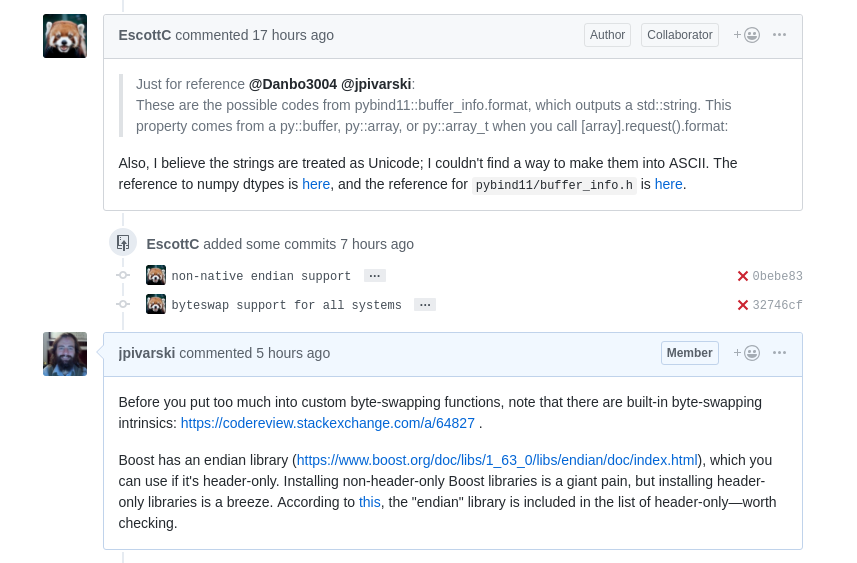
\includegraphics[width=0.9\linewidth]{awkward-cpp-ongoing.png}
\end{center}
\end{frame}

\begin{frame}{awkward-numba: my primary coding project; last touched Feb 27}
\vspace{0.25 cm}

\begin{columns}[t]
\column{0.5\linewidth}
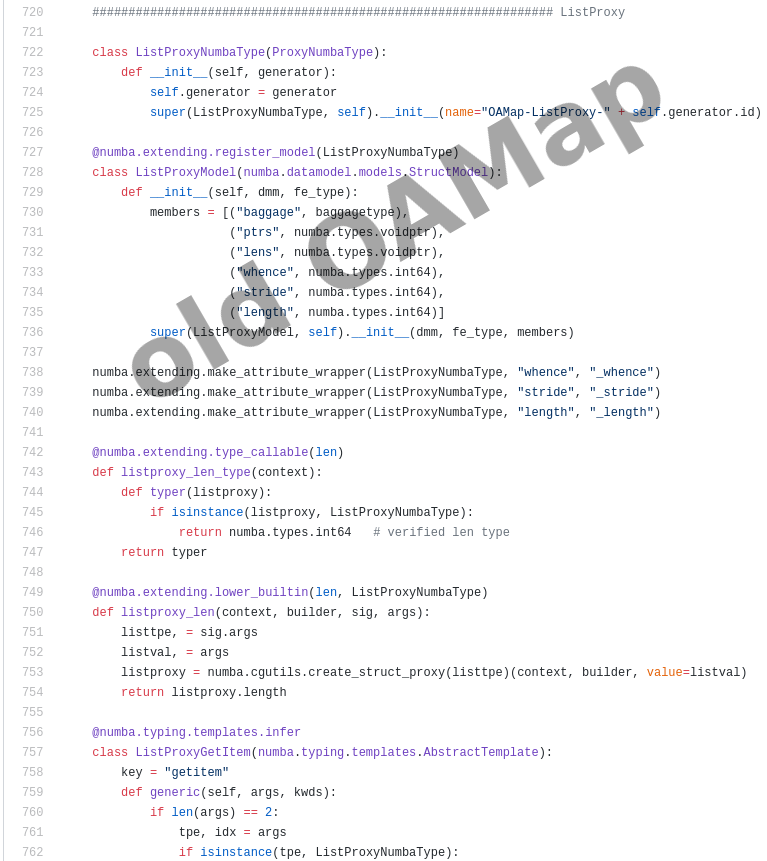
\includegraphics[width=\linewidth]{numbafied-oamap.png}

\column{0.51\linewidth}
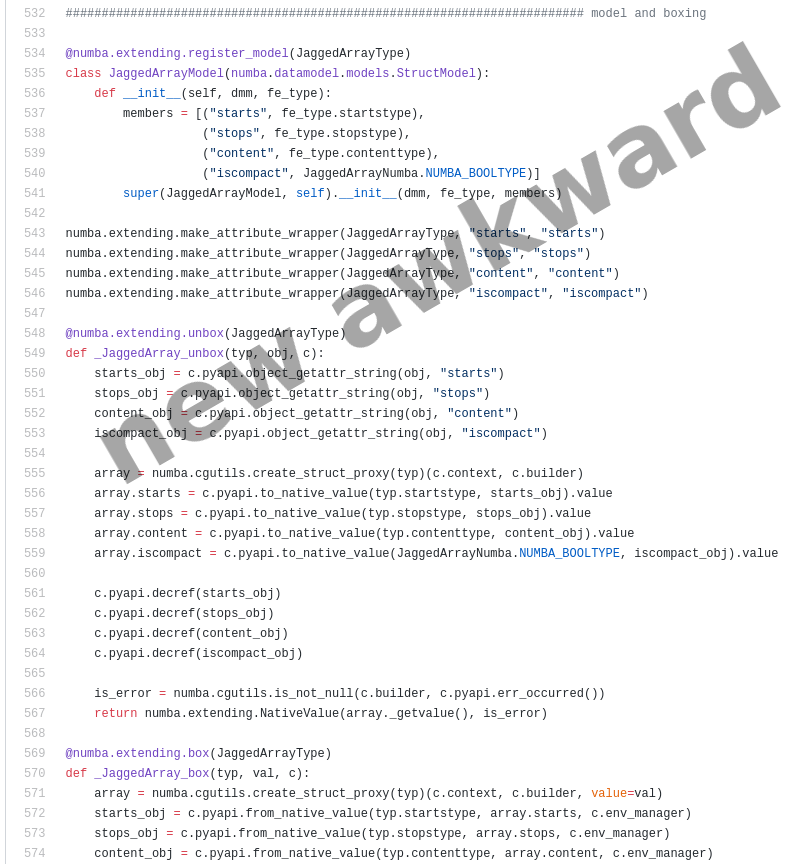
\includegraphics[width=\linewidth]{numbafied-awkward.png}
\end{columns}
\end{frame}

\begin{frame}{Histogramming ergonomics}
\vspace{-0.04 cm}

\begin{center}
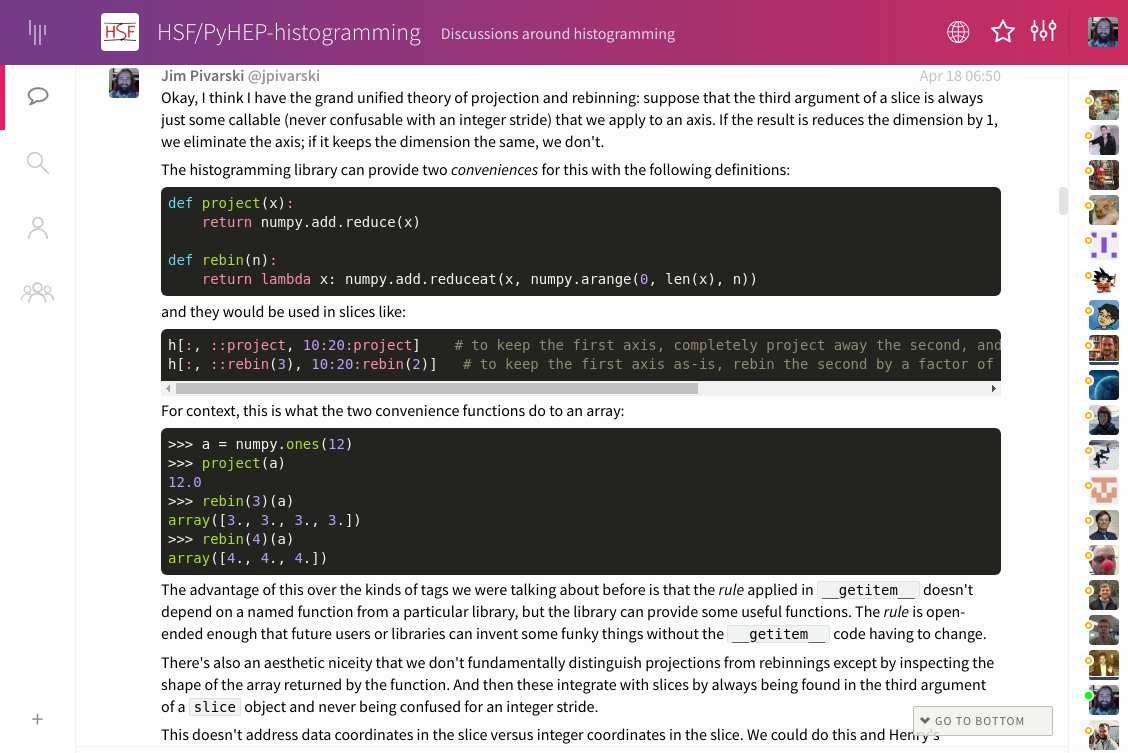
\includegraphics[width=0.85\linewidth]{gitter-histogramming.png}
\end{center}
\end{frame}

\begin{frame}[fragile]{Toy languages: pattern matching for particle combinatorics}
\small
\begin{minted}{swift}
higgs(flavor1, flavor2) =       // define a join pattern in a function
    join {
        z1 ~ {                  // Z boson subpattern
            lep1 ~ flavor1      // lep1, lep2 from flavor1 collection
            lep2 ~ flavor1      // leptons are NOT double-counted
            mass = (lep1.p4 + lep2.p4).mass
        }
        z2 ~ {                  // another Z boson
            lep1 ~ flavor2      // lep1, lep2 from flavor2, which
            lep2 ~ flavor2      // might be the same as flavor1
            mass = (lep1.p4 + lep2.p4).mass
        }                       // filter and sort with functionals
    }.filter(h => h.z1.lep1.charge != h.z1.lep2.charge and
                  h.z2.lep1.charge != h.z2.lep2.charge)
     .sort(h => (h.z1.mass - 91)**2 + (h.z2.mass - 91)**2)
\end{minted}
\begin{minted}{swift}
higgs4e    = higgs(electrons, electrons)    // use the function
higgs4mu   = higgs(muons, muons)            // to match patterns
higgs2e2mu = higgs(electrons, muons)
\end{minted}
\end{frame}

\begin{frame}{Laurelin: uproot-like ROOT I/O in Java}
\begin{center}
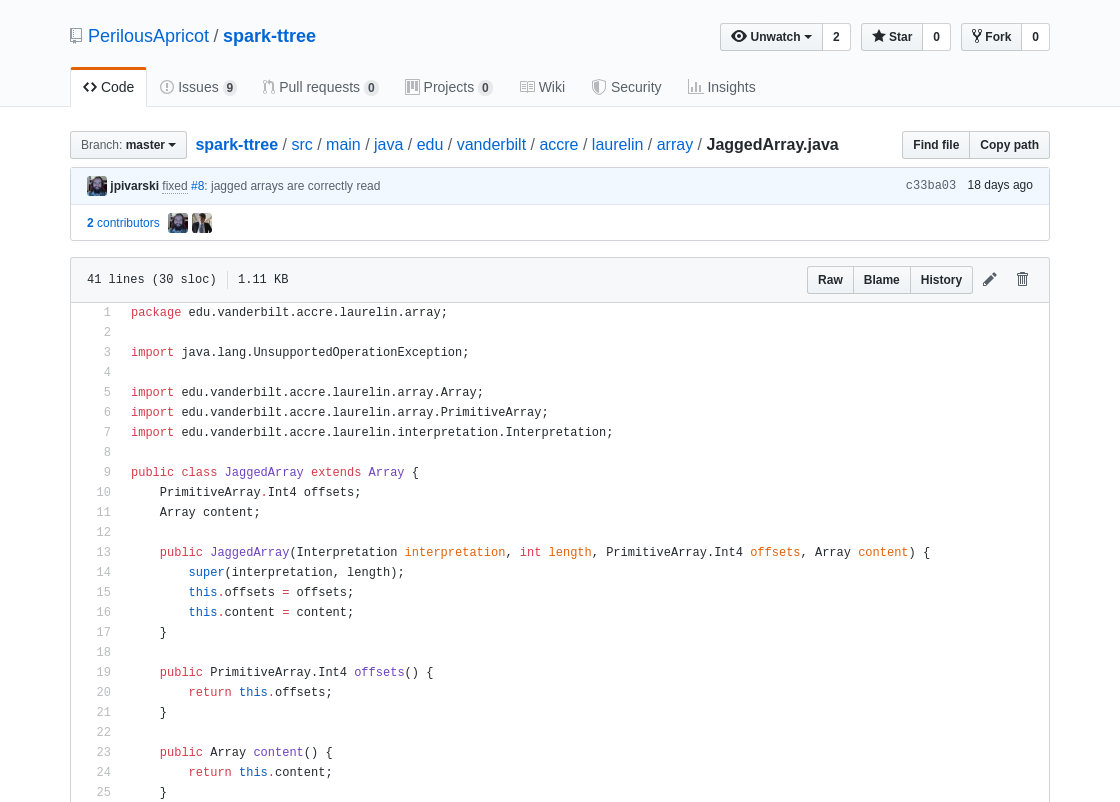
\includegraphics[width=\linewidth]{laurelin-jaggedarray.png}
\end{center}
\end{frame}

\begin{frame}[fragile]{uproot $\to$ SkyHook}
\scriptsize
\begin{columns}[t]
\column{0.5\linewidth}
\begin{minted}{protobuf}
include "interpretation.fbs";

enum Compression: int {
  none = 0,
  zlib = 1,
  lzma = 2,
  old = 3,
  lz4 = 4
}

table Branch {
  local_offsets: [ulong] (required);
  page_seeks: [ulong] (required);
  compression: Compression;
  iscompressed: [bool];
  compressedbytes: [uint];
  uncompressedbytes: [uint] (required);
  basket_page_offsets: [uint] (required);
  basket_keylens: [uint];
  basket_data_borders: [uint];
}
\end{minted}

\column{0.5\linewidth}
\begin{minted}{protobuf}
table Column {
  interp: uproot_skyhook
      .interpretation_generated
      .Interpretation (required);
  title: string;
}

table File {
  location: string (required);
  uuid: string (required);
  branches: [Branch] (required);
}

table Dataset {
  name: string (required);
  treepath: string (required);
  colnames: [string] (required);
  columns: [Column] (required);
  files: [File] (required);
  global_offsets: [ulong] (required);
  location_prefix: string;
}
\end{minted}

\end{columns}
\end{frame}

\begin{frame}{\cancel{RForest} RNtuple discussions}
\vspace{-0.04 cm}

\begin{center}
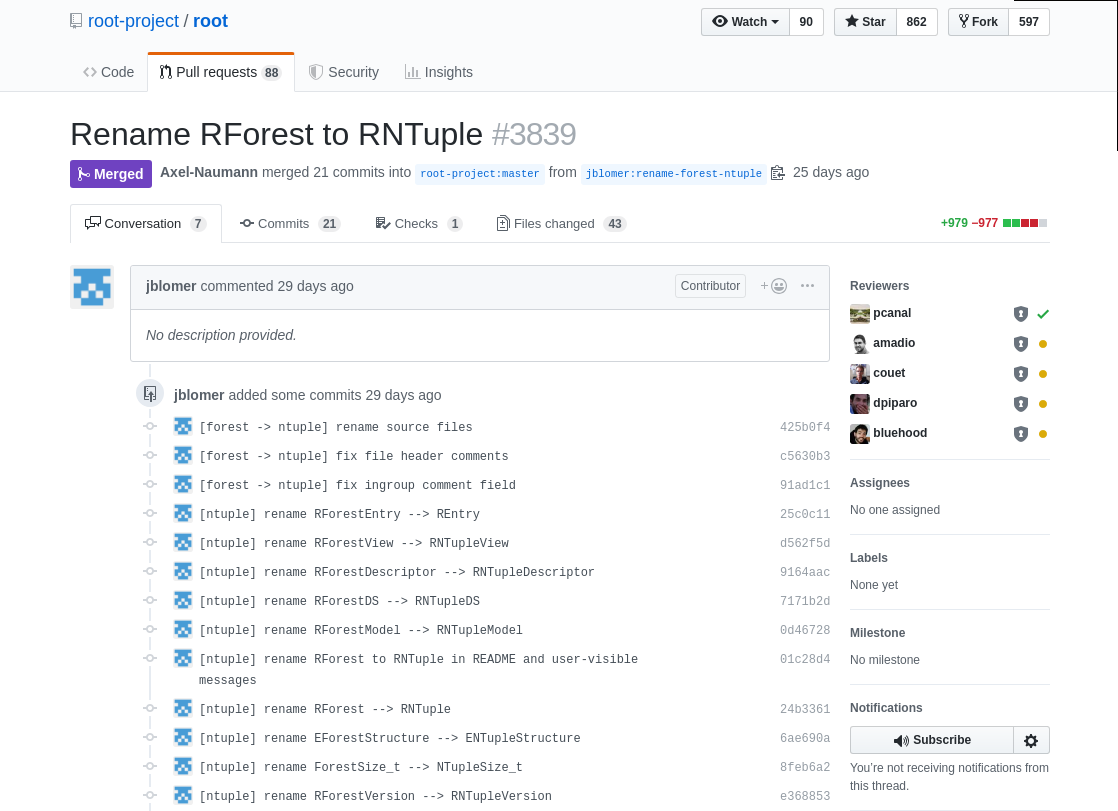
\includegraphics[width=0.85\linewidth]{rforest-rntuple.png}
\end{center}
\end{frame}

\end{document}
